\section{Interface Homme-Machine}

\subsection{Introduction}

La fonction principale de l’application est de valider les transcriptions d’un document.
Nous.décrivons ici par document un fichier manuscrit ou imprimé scanné composé d’une ou plusieurs pages. L’application propose ainsi de valider un ensemble d’annotations
(\textbf{PEA\_GEN\_1}), d’éditer manuellement les transcriptions
(\textbf{PEA\_GEN\_2}), ou encore de corriger les annotations proposées par un
reconnaisseur externe à l’application (\textbf{PEA\_GEN\_3}).

\paragraph{}
Le couple imagette-transcription est chargé depuis la base de données. Lorsque
la vérité-terrain d’une imagette est modifiée, les modifications sont aussitôt
envoyées à la base de données (\textbf{PEA\_GEN\_4}). En outre, si une
imagette ou sa transcription n’est pas pertinente pour l’ensemble
d’apprentissage, le couple peut être ignoré à l’aide d’un bouton prévu à cet
effet (\textbf{PEA\_GEN\_5}). Cette fonctionnalité sera expliquée plus en
détail par la suite.

\paragraph{}
Les documents sont regroupés en projets (par exemple, l’ensemble des registres
paroissiaux de 1800 à 1810) (\textbf{PEA\_GEN\_6}). En ouvrant l’application,
l’utilisateur sélectionne d’abord le projet puis le document sur lequel il
veut travailler et enfin le mode dans lequel il veut ouvrir le document 
(annotation manuelle, correction des propositions du reconnaisseur ou validation 
des transcriptions) (\textbf{PEA\_GEN\_7}). Les documents sont simplement décrits 
par leur nom (par exemple, “Registre Paroissial de la commune de Bécherel de 
1800 à 1810).  Il peut également créer un nouveau
projet (\textbf{PEA\_GEN\_8}). Pour ce faire, l’utilisateur clique sur le 
bouton “Nouveau projet”, le nomme, puis le remplit en choisissant parmi 
ses fichiers les manuscrits qu’il contiendra.

\paragraph{}
Une fois que l’utilisateur a choisi le document sur lequel il veut travailler, il 
peut basculer vers la page de découpe des zones (\textbf{PEA\_GEN\_9}), vers
la page d’édition des annotations (\textbf{PEA\_GEN\_10}) ou bien vers la page
de validation des transcriptions (\textbf{PEA\_GEN\_11}).

\paragraph{}
\begin{mdframed}[frametitle={Figure 6 : Accueil de l'application}, innerbottommargin=10]
\begin{center}
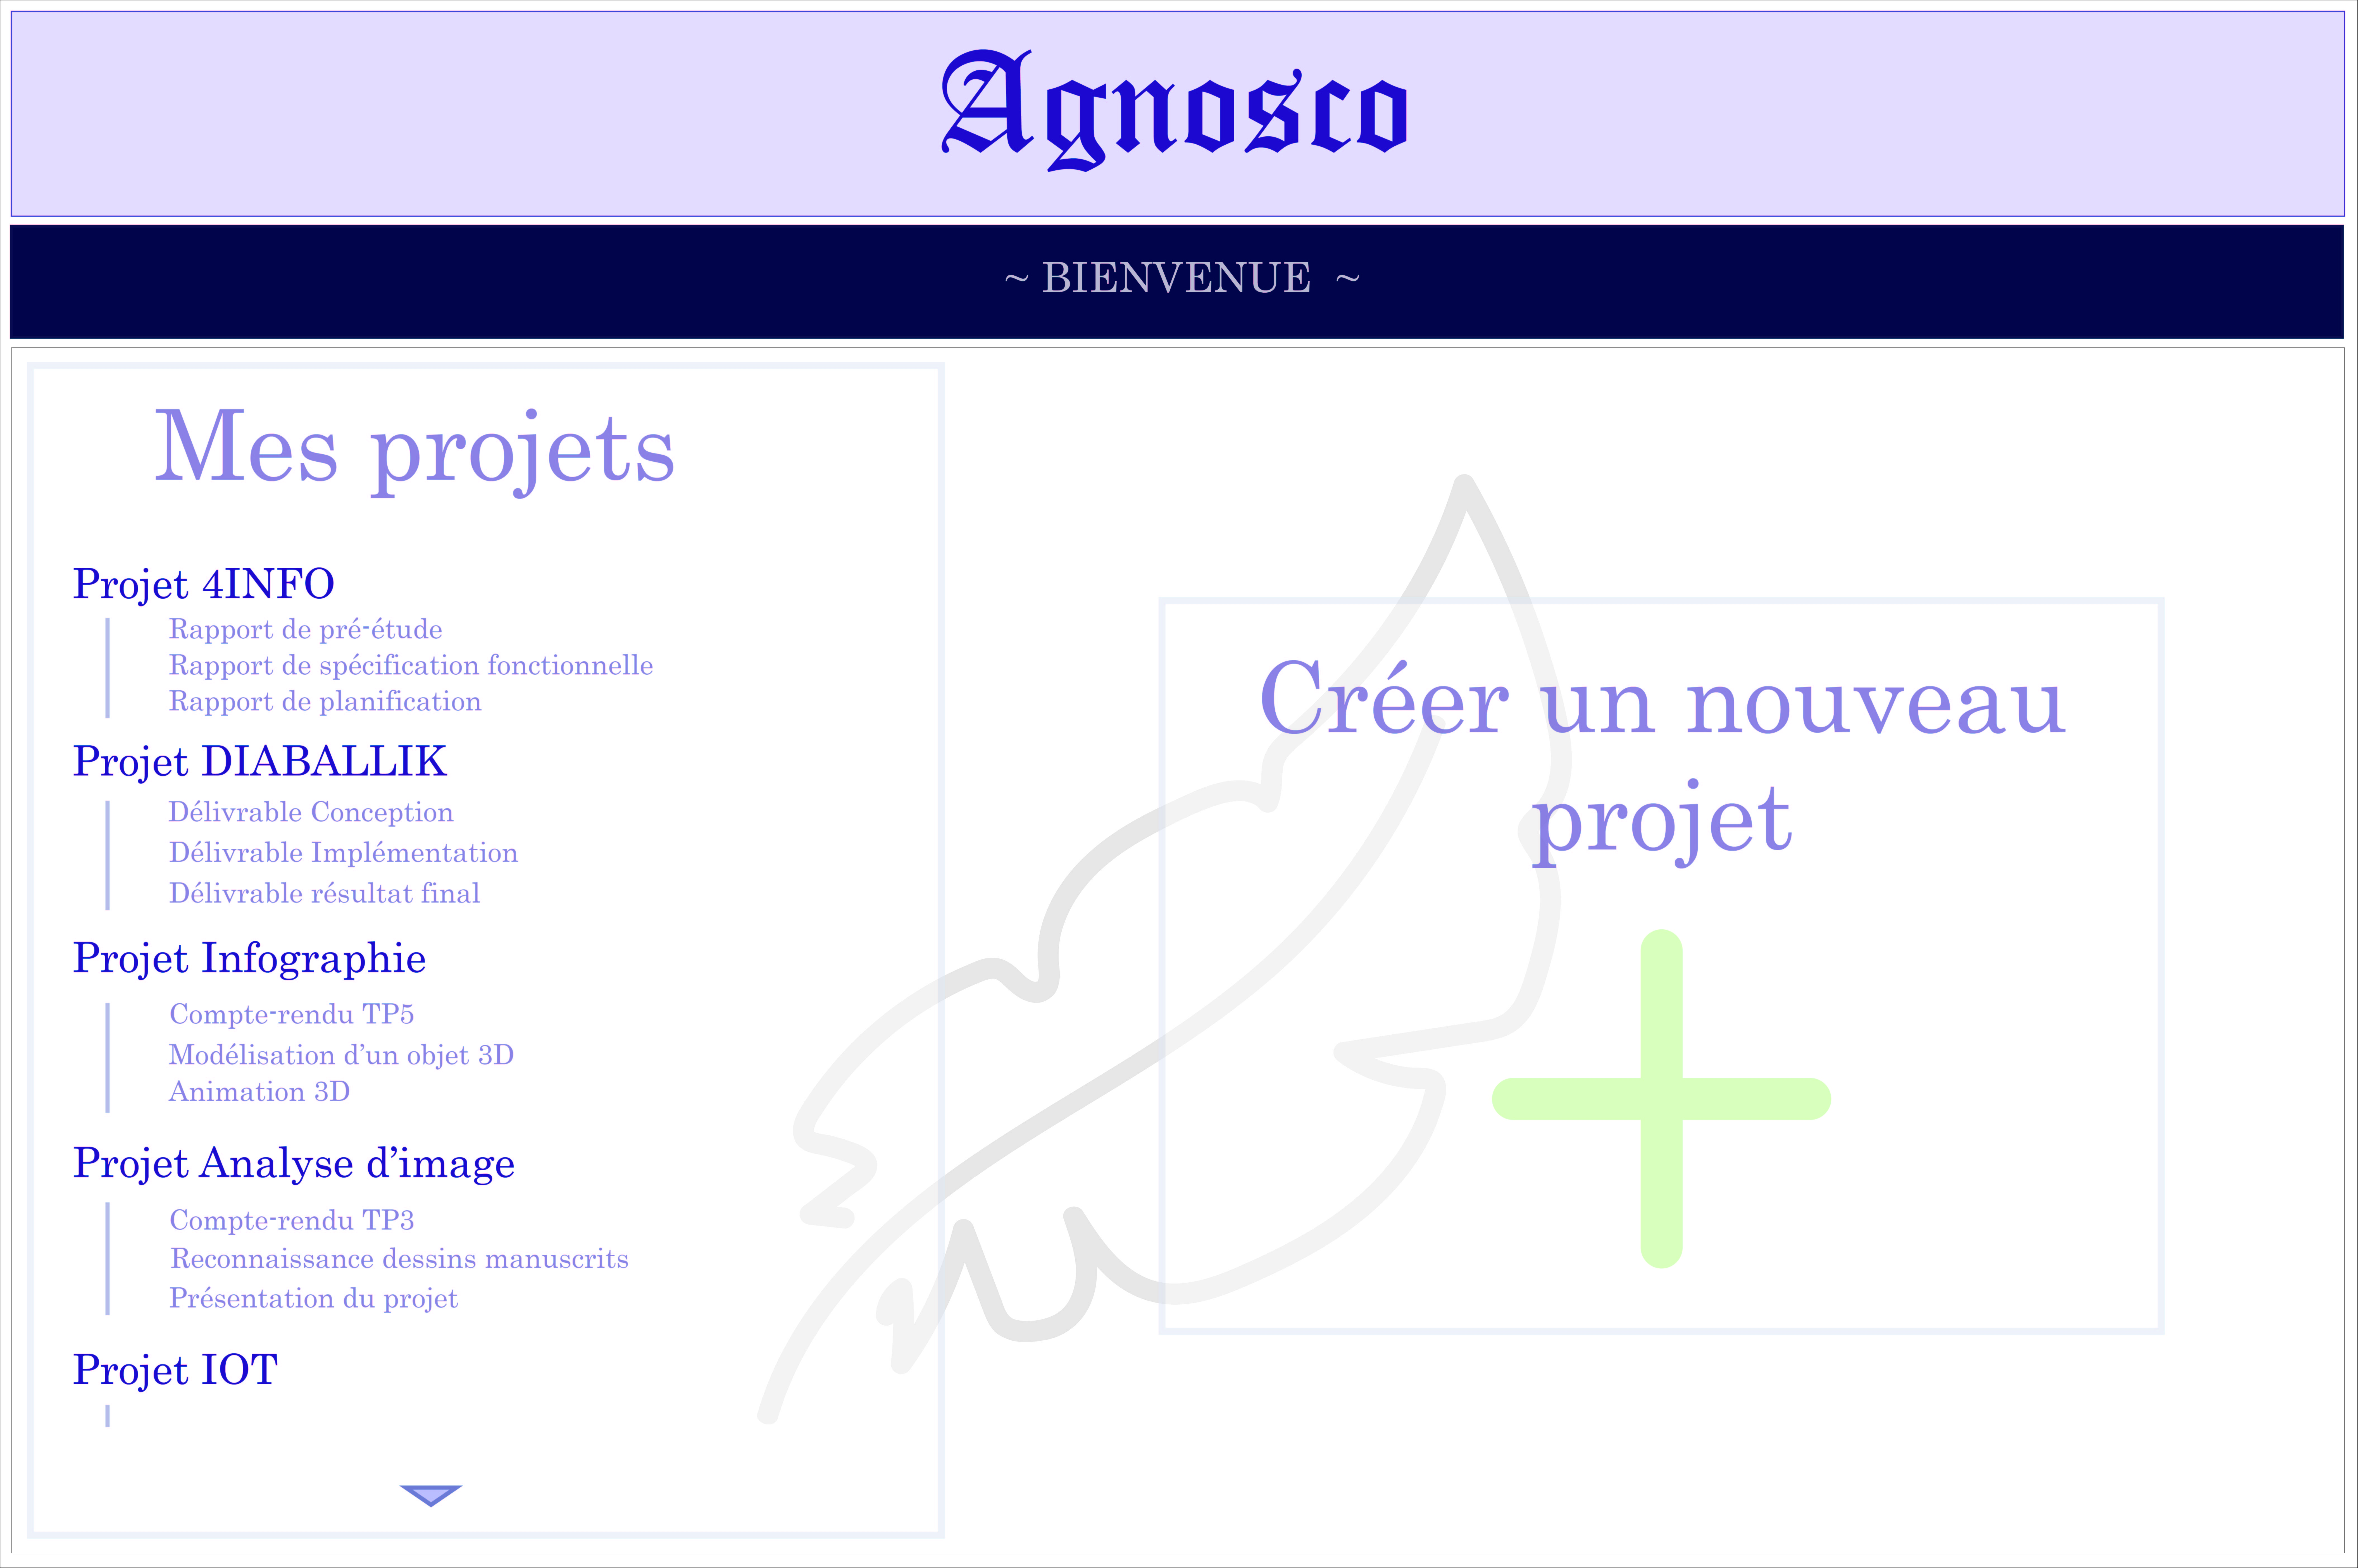
\includegraphics[scale=0.05]{ihm1.jpg}
\end{center}
\end{mdframed}

\subsection{Page de découpe des zones}

Cette page permet à l’utilisateur de définir et de modifier les différentes
zones qui découpent le document. La page d’édition des zones offre
plusieurs outils de découpe, d’édition des zones et de navigation dans le
document. L’outil “nouvelle sélection” crée une nouvelle zone à l’aide d’un
rectangle (\textbf{PDEC\_OD\_1}). Les rectangles qui définissent initialement
les zones doivent avoir des sommets dont on peut modifier la position pour
une découpe plus fine (\textbf{PDEC\_OD\_2}). De plus, l’utilisateur doit avoir
la possibilité de rajouter des sommets à la zone (\textbf{PDEC\_OD\_3}). Les
zones ne sont donc pas limitées à des rectangles, mais peuvent prendre la forme
d’autres polygones. Lorsqu’une nouvelle zone est créée, elle se voit attribuée
le type par défaut “Corps de texte”. L’utilisateur peut changer son type avec
un menu déroulant (\textbf{PDEC\_OD\_4}). Chaque zone possède un type car
l’apprentissage du reconnaisseur se fera différemment selon si la zone contient
un corps de texte ou un titre, par exemple.

\paragraph{}
L’outil “déplacer” déplace la zone sélectionnée sur le document
(\textbf{PDEC\_OD\_5}). Cela est utile quand l’utilisateur s’aperçoit que
plusieurs de ses zones sont mal positionnées. Il peut donc déplacer chaque zone
en un clic à l’aide de cet outil. L’outil “zoom +” permet de zoomer sur le
document et “zoom -” de dézoomer, afin de faciliter l’édition des zones, pour
une meilleure ergonomie (\textbf{PDEC\_OD\_6}). L’outil “annuler” permet
d’annuler la dernière action (\textbf{PDEC\_OD\_7}) et l’outil “refaire” permet
de refaire l’action annulée précédemment (\textbf{PDEC\_OD\_8}). L’outil
“réinitialiser” supprime toutes les zones de la page pour retourner au
document vierge (\textbf{PDEC\_OD\_9}) en cas de travail erroné. Cela évite à
l’utilisateur d’avoir à supprimer les zones une par une.

\paragraph{}
Afin de permettre à l’utilisateur de vérifier son travail au fur et à mesure,
l’interface de découpe doit proposer un outil “appliquer la détection de
lignes sur la zone” (\textbf{PDEC\_OD\_10}). Cet outil applique le détecteur de
lignes sur la zone sélectionnée, afin de voir quelles lignes sont détectées
pour vérifier que la zone est bien définie. Lorsque l’utilisateur a fini la
découpe d’une page, trois possibilités s’offrent à lui. Il peut tout d’abord
choisir de continuer la découpe du document sur la page suivante
(\textbf{PDEC\_OD\_11}), de passer à l’édition des annotations sur la page qu’il
vient de découper (\textbf{PDEC\_OD\_12}) ou bien d’exporter la page découpée au
format PiFF afin de soumettre les données à un reconnaisseur externe à
l’application (\textbf{PDEC\_OD\_13}).

\paragraph{}
Enfin, l’interface doit posséder un bouton de retour au menu principal
(\textbf{PDEC\_OD\_14}). De plus, la zone de visualisation doit pouvoir permettre
à l’utilisateur de se déplacer sur le document à l’aide d’un \textit{scroll} horizontal
et vertical (\textbf{PDEC\_OD\_15}).

\newpage

\begin{mdframed}[frametitle={Figure 7 : Édition des zones de découpe}, innerbottommargin=10]
\begin{center}
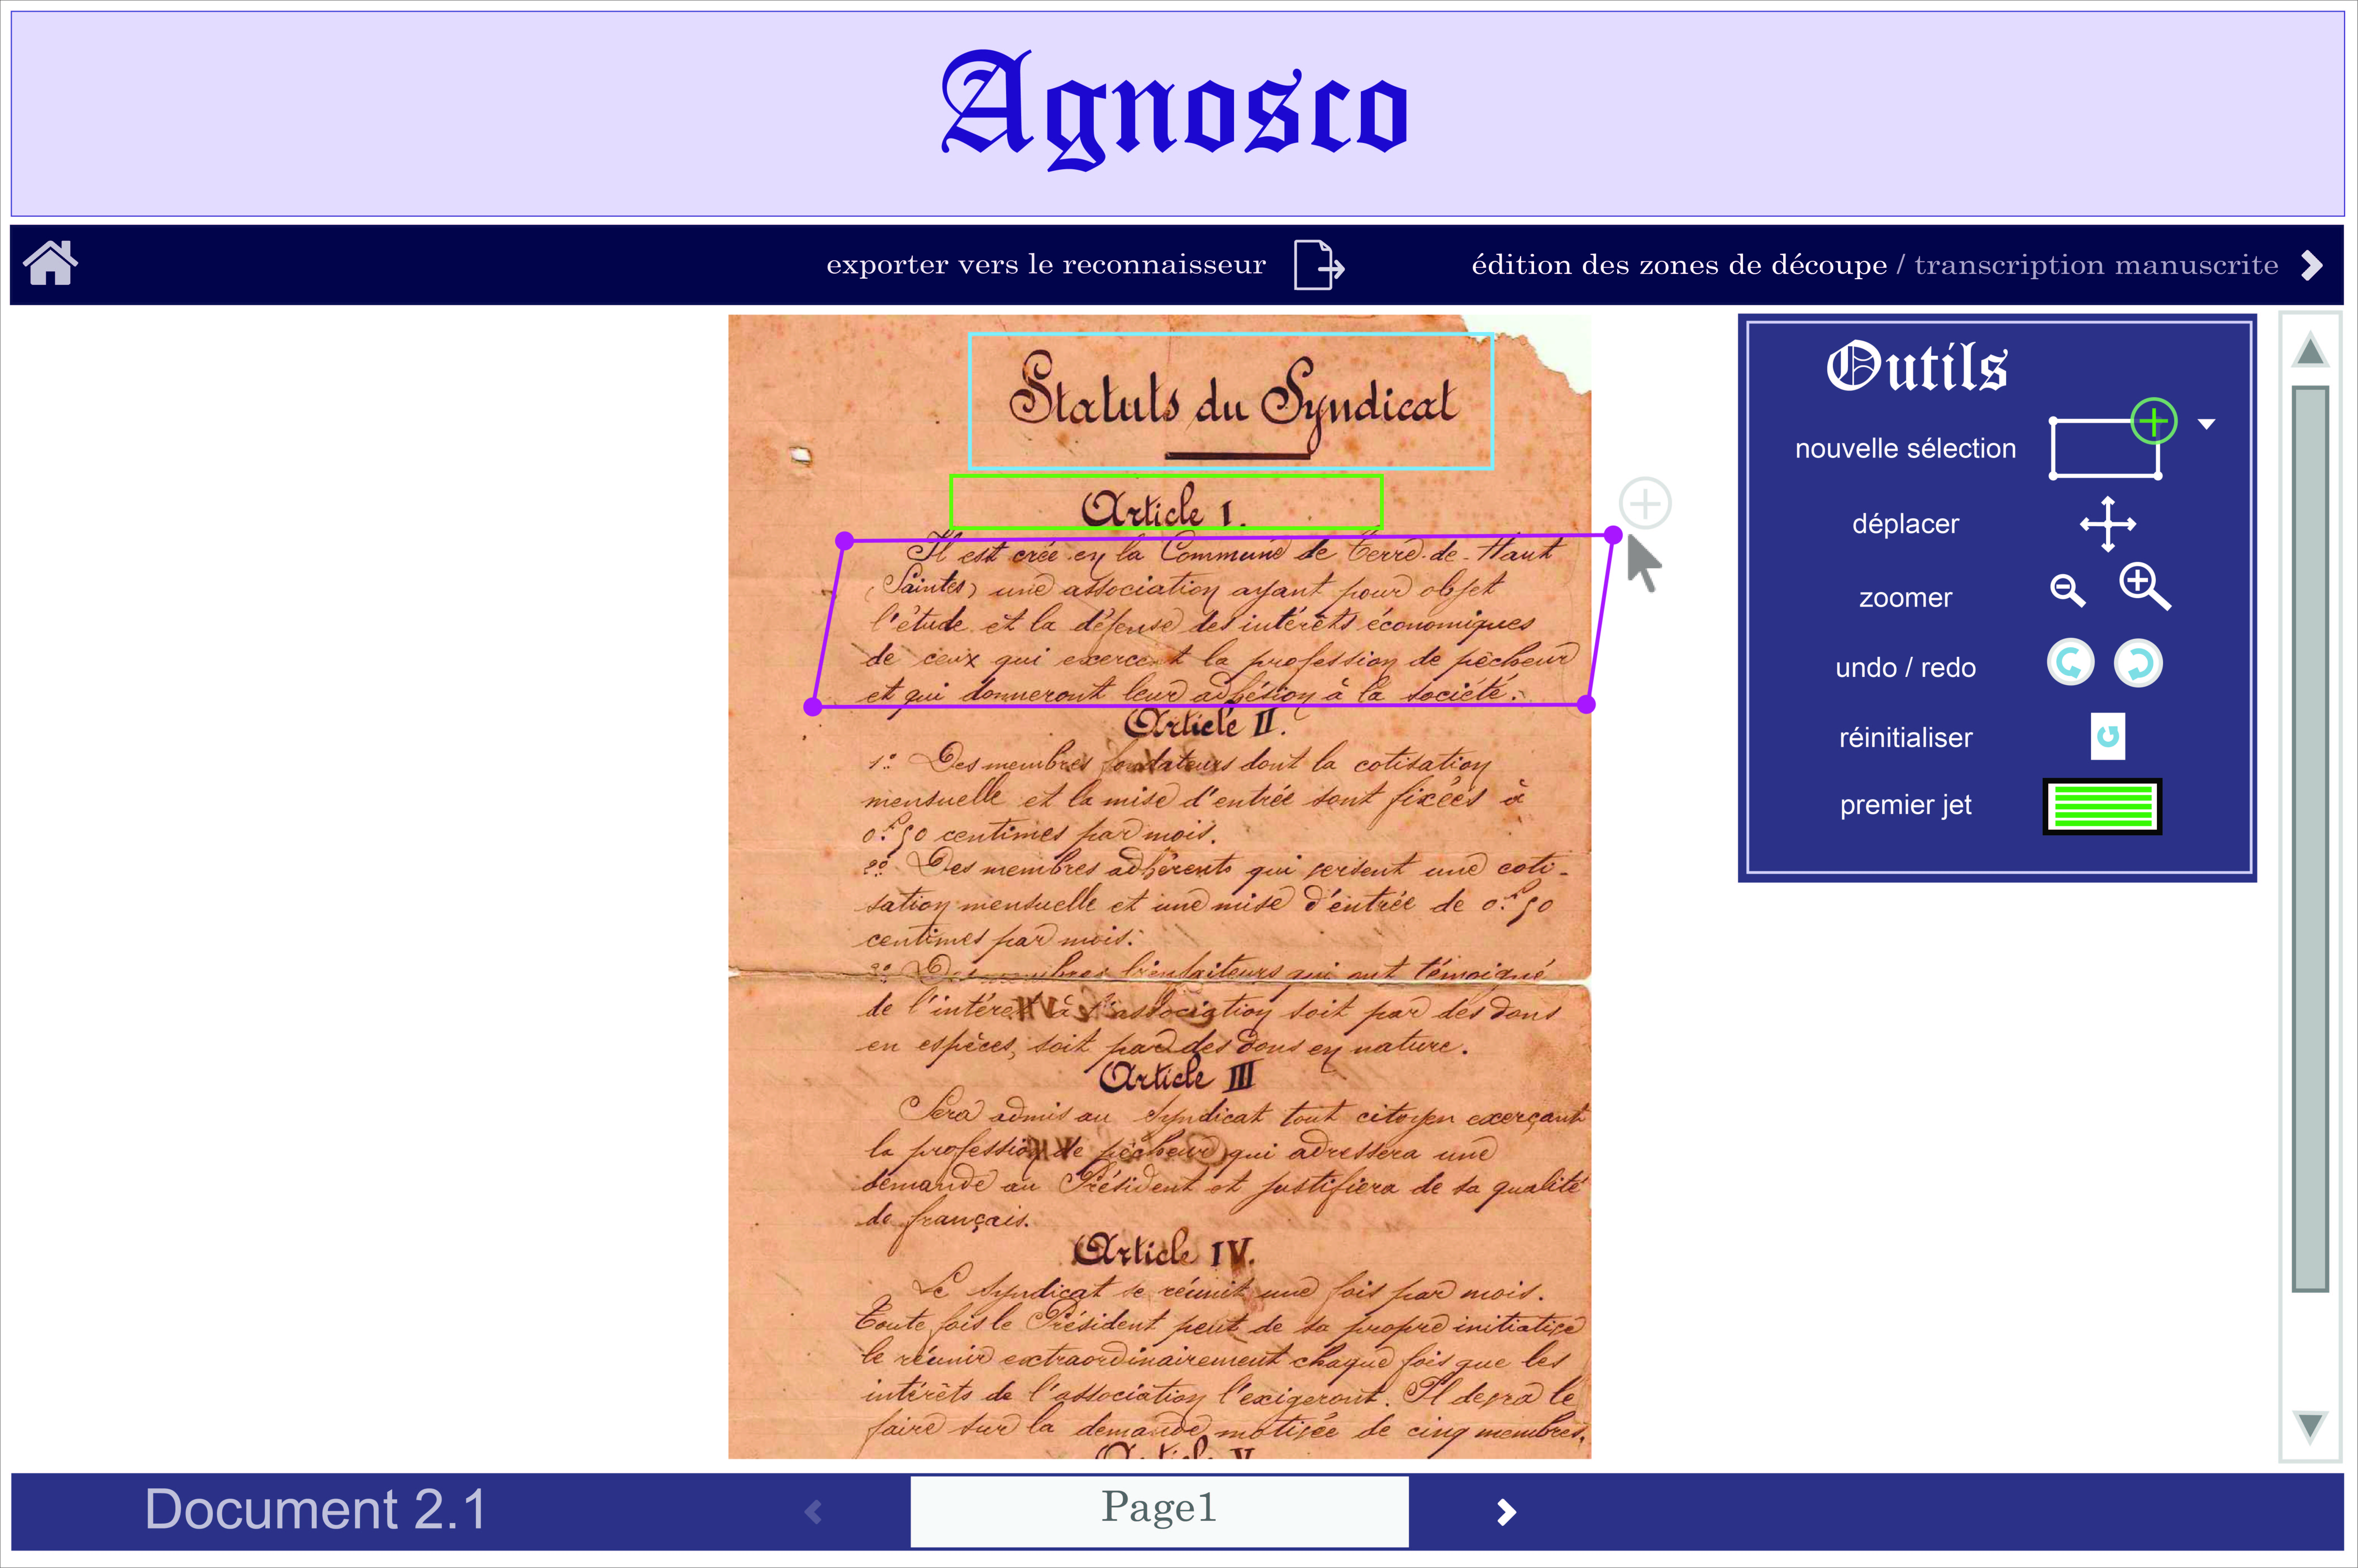
\includegraphics[scale=0.05]{ihm2.jpg}
\end{center}
\end{mdframed}

\subsection{Page d'édition manuelle des annotations}

Cette page permet à l’utilisateur de rédiger manuellement les transcriptions
afin de générer l’ensemble d’apprentissage. Pour faciliter le travail de
l’utilisateur, à l’ouverture de la page, le curseur est placé sur la première
imagette ne possédant pas de transcription (\textbf{PEMA\_1}). Puis, pendant
l’édition des vérités-terrain, un simple appui sur la touche Entrée permet de
positionner le curseur sur l’annotation suivante afin de faciliter la
navigation et de réduire le temps passé à l’édition des transcriptions
(\textbf{PEMA\_2}). L’utilisateur peut naviguer entre les zones grâce à 
la barre dédiée en bas de la fenêtre. Enfin, l’interface doit proposer un raccourci clavier
permettant de basculer vers la prochaine imagette sans vérité-terrain
(\textbf{PEMA\_3}). Cela est utile dans le cas où les transcriptions manquantes
sont éparpillées et ne se suivent pas. Comme c’est une fonctionnalité qui ne
sera pas forcément utilisée très souvent, nous avons opté pour un raccourci
clavier plutôt qu’un bouton pour éviter de surcharger l’interface.

\paragraph{}
Sur cette page, l’utilisateur a toujours la possibilité de basculer vers la
page d’édition des zones de découpe. L’interface doit donc posséder un bouton
intitulé “modifier les zones du manuscrit” (\textbf{PEMA\_4}). La zone
principale de l’interface doit afficher la liste des imagettes du document
découpé (\textbf{PEMA\_5}). Chaque imagette est suivie de l’annotation
correspondante. Nous avons choisi de présenter le document en séparant les
imagettes les unes des autres pour améliorer la lisibilité du texte et des
transcriptions ligne par ligne. De plus, cette présentation nous permet quand
même d’avoir accès au contexte de la ligne courante, c’est-à-dire les imagettes
précédente et suivante. Enfin, avec une telle séparation des imagettes,
l’utilisateur peut vérifier que la détection des lignes a été bien effectuée
et que les imagettes sont découpées correctement.

\paragraph{}
Si un couple imagette-transcription ne semble pas pertinent pour l’étude, une
croix permet de le griser afin qu’il soit ignoré (\textbf{PEMA\_6}). Il ne sera
pas supprimé de la base de données, mais si un reconnaisseur est utilisé sur
le document, le couple ignoré ne sera pas pris en compte par celui-ci.
L’utilisateur garde la possibilité de le dégriser en cliquant sur la flèche
orange dans le coin droit de l’imagette. Enfin, l’utilisateur peut basculer
vers la page de validation des transcriptions afin de valider et d’exporter son
travail (\textbf{PEMA\_7}).

\paragraph{}
\begin{mdframed}[frametitle={Figure 8 : Transcription manuscrite}, innerbottommargin=10]
\begin{center}
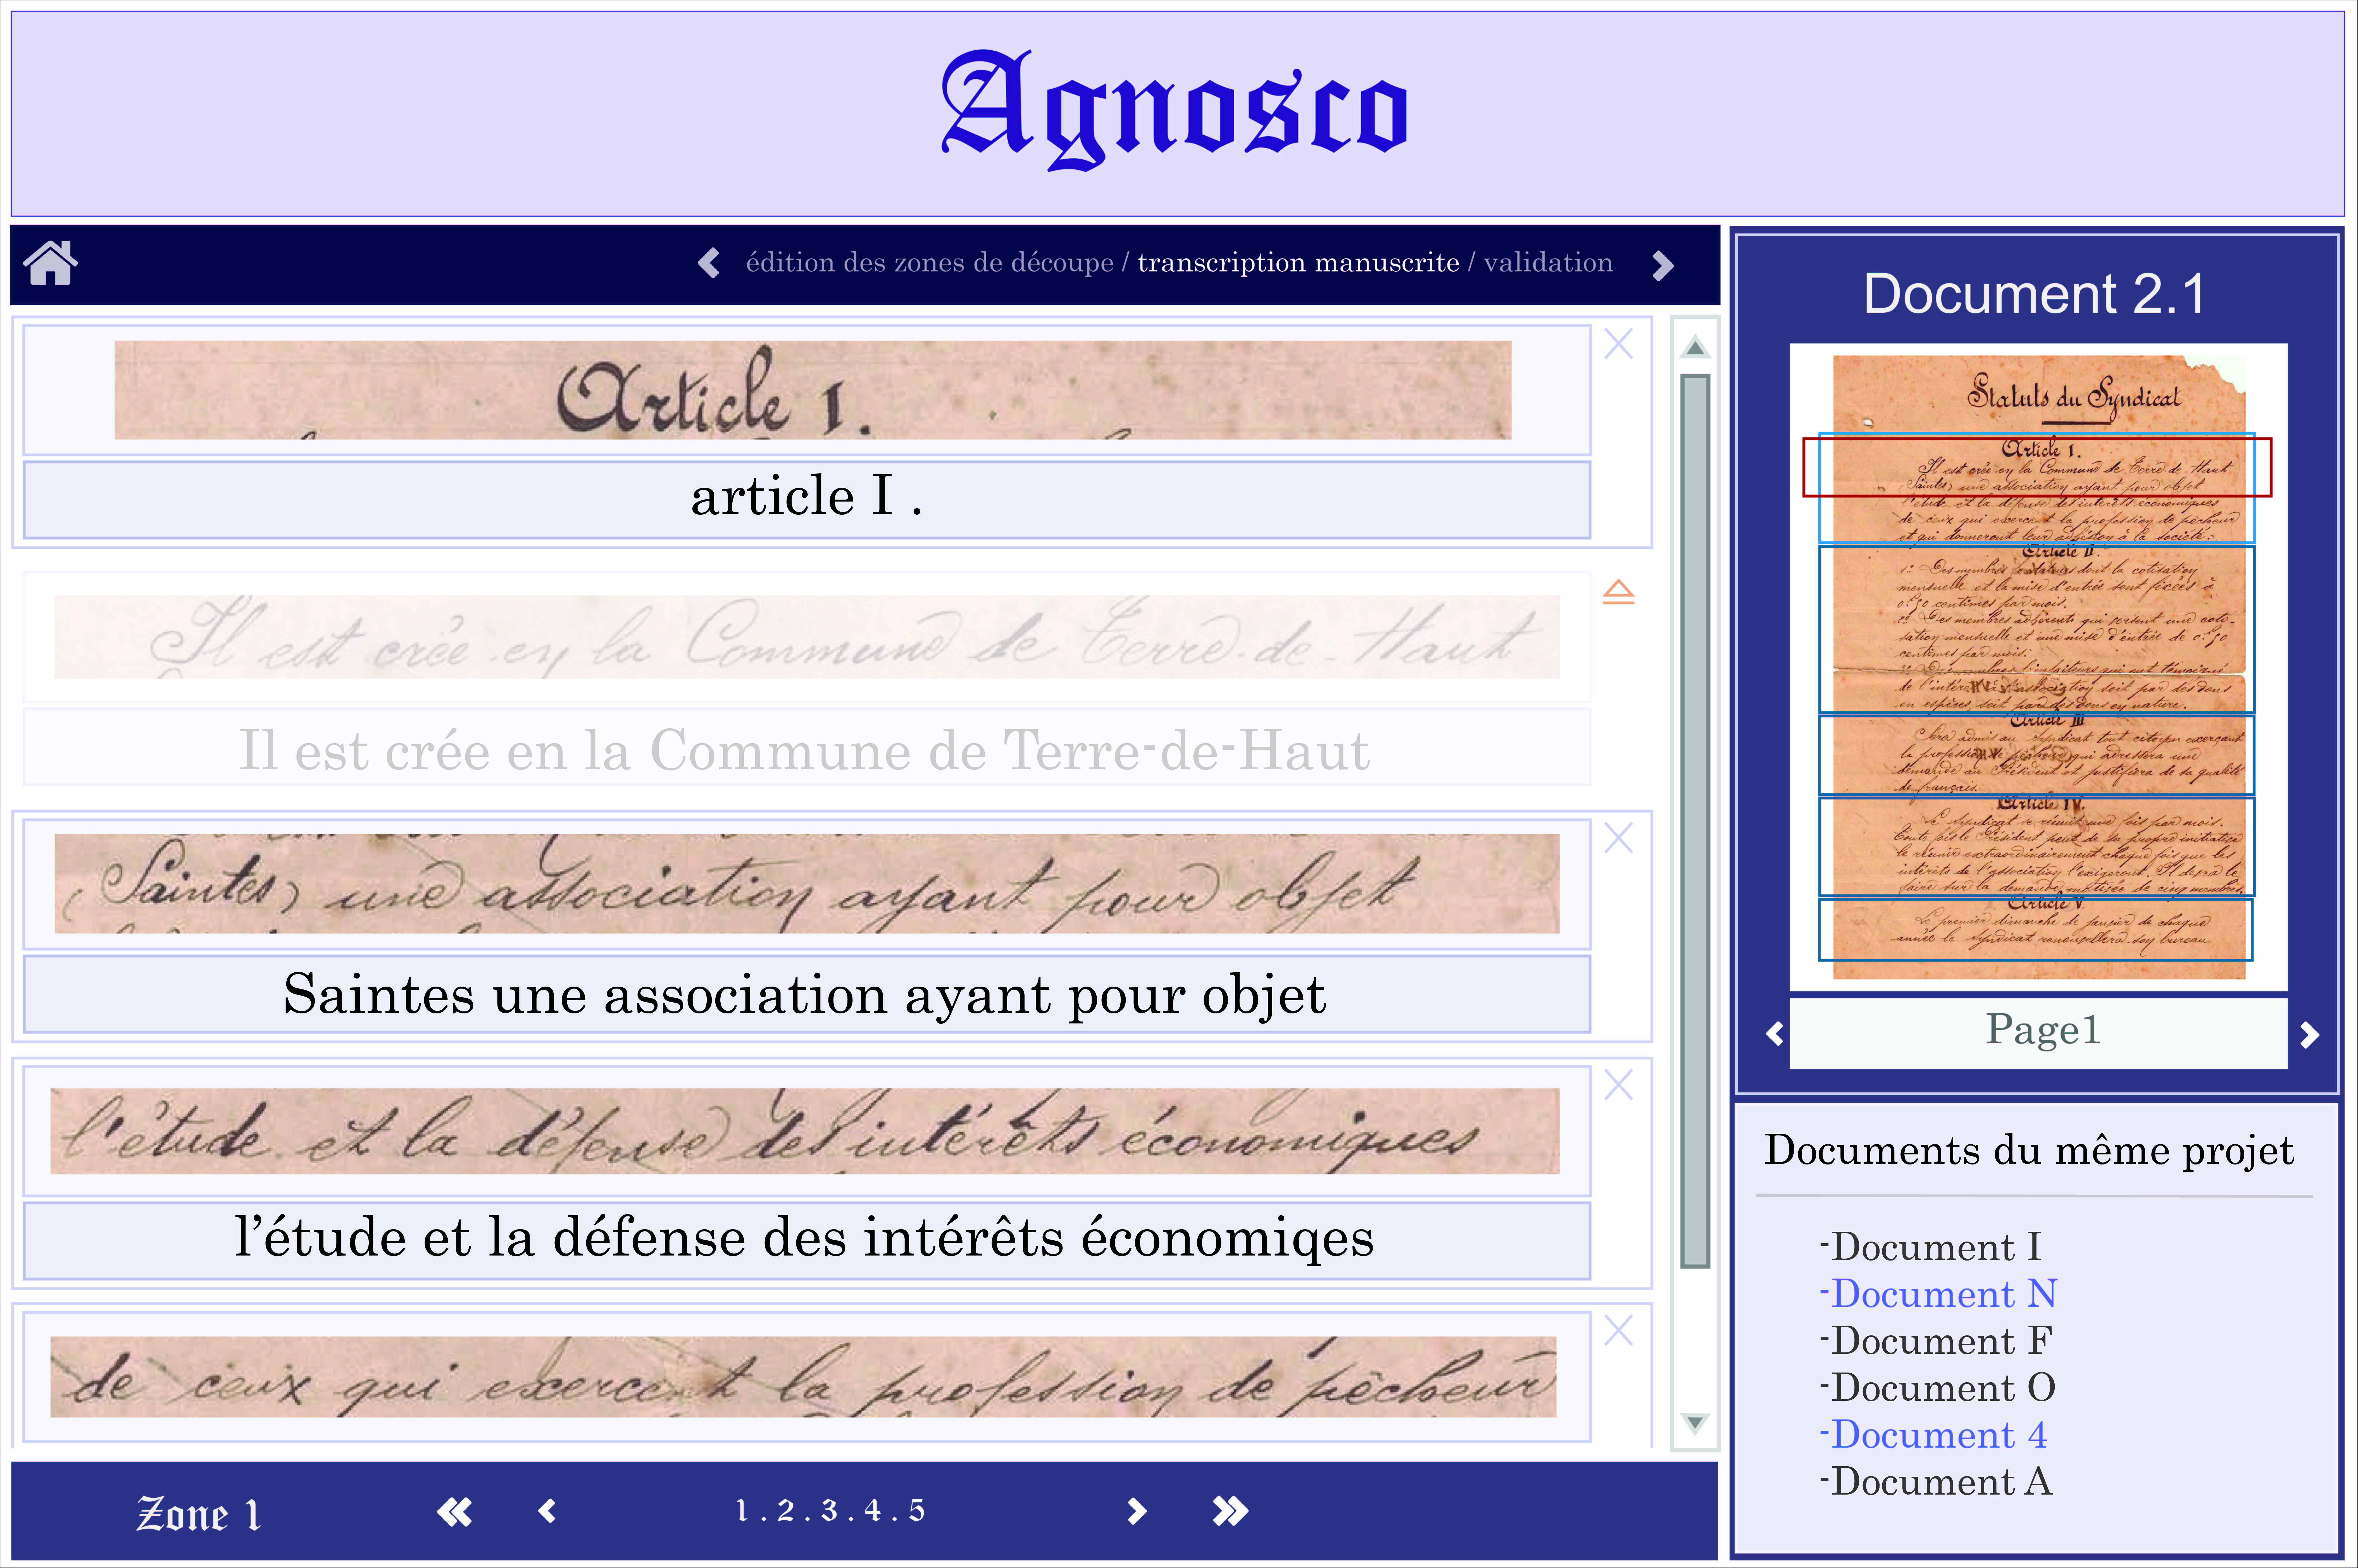
\includegraphics[scale=0.05]{ihm3.jpg}
\end{center}
\end{mdframed}

\subsection{Page de correction des transcriptions du reconnaisseur}

Si l’utilisateur a fait passer un document par un reconnaisseur d’écriture
manuscrite, il veut pouvoir visualiser le résultat qui fait suite à son
apprentissage et le corriger manuellement si besoin. C’est ce que permet
cette page de l’interface. Celle-ci est semblable à la page d’édition manuelle
des annotations car son fonctionnement est sensiblement le même à quelques
fonctionnalités près.

\paragraph{}
En partant du principe que les transcriptions proposées par l’IA sont
relativement fiables et pour diminuer le temps passé à la validation, un simple
appui sur Entrée valide les transcriptions zone par zone et passe à la zone
suivante (\textbf{PCORIA\_1}). Si une transcription est fausse, l’utilisateur
doit pouvoir la modifier en cliquant dessus pour y positionner son curseur et
en effectuant ses modifications manuellement (\textbf{PCORIA\_2}).

\paragraph{}
La zone de visualisation des imagettes se présente de la même manière que sur
la page d’édition manuelle des transcriptions (\textbf{PCORIA\_3}). De même, 
l’utilisateur peut naviguer entre les zones grâce à la barre de navigation en 
bas de la fenêtre. Il peut également naviguer entre les pages du document grâce 
aux flèches dans la zone à droite des imagettes où figurela page courante 
en entier. Cette page
possède également la fonctionnalité de mise à l’écart d’un couple
imagette-transcription, comme dans la page précédente (\textbf{PCORIA\_4}).
Enfin, l’utilisateur peut également basculer vers la page de validation des
transcriptions afin de valider et d’exporter son travail (\textbf{PCORIA\_5}).

\newpage

\begin{mdframed}[frametitle={Figure 9 : Correction de l'IA}, innerbottommargin=10]
\begin{center}
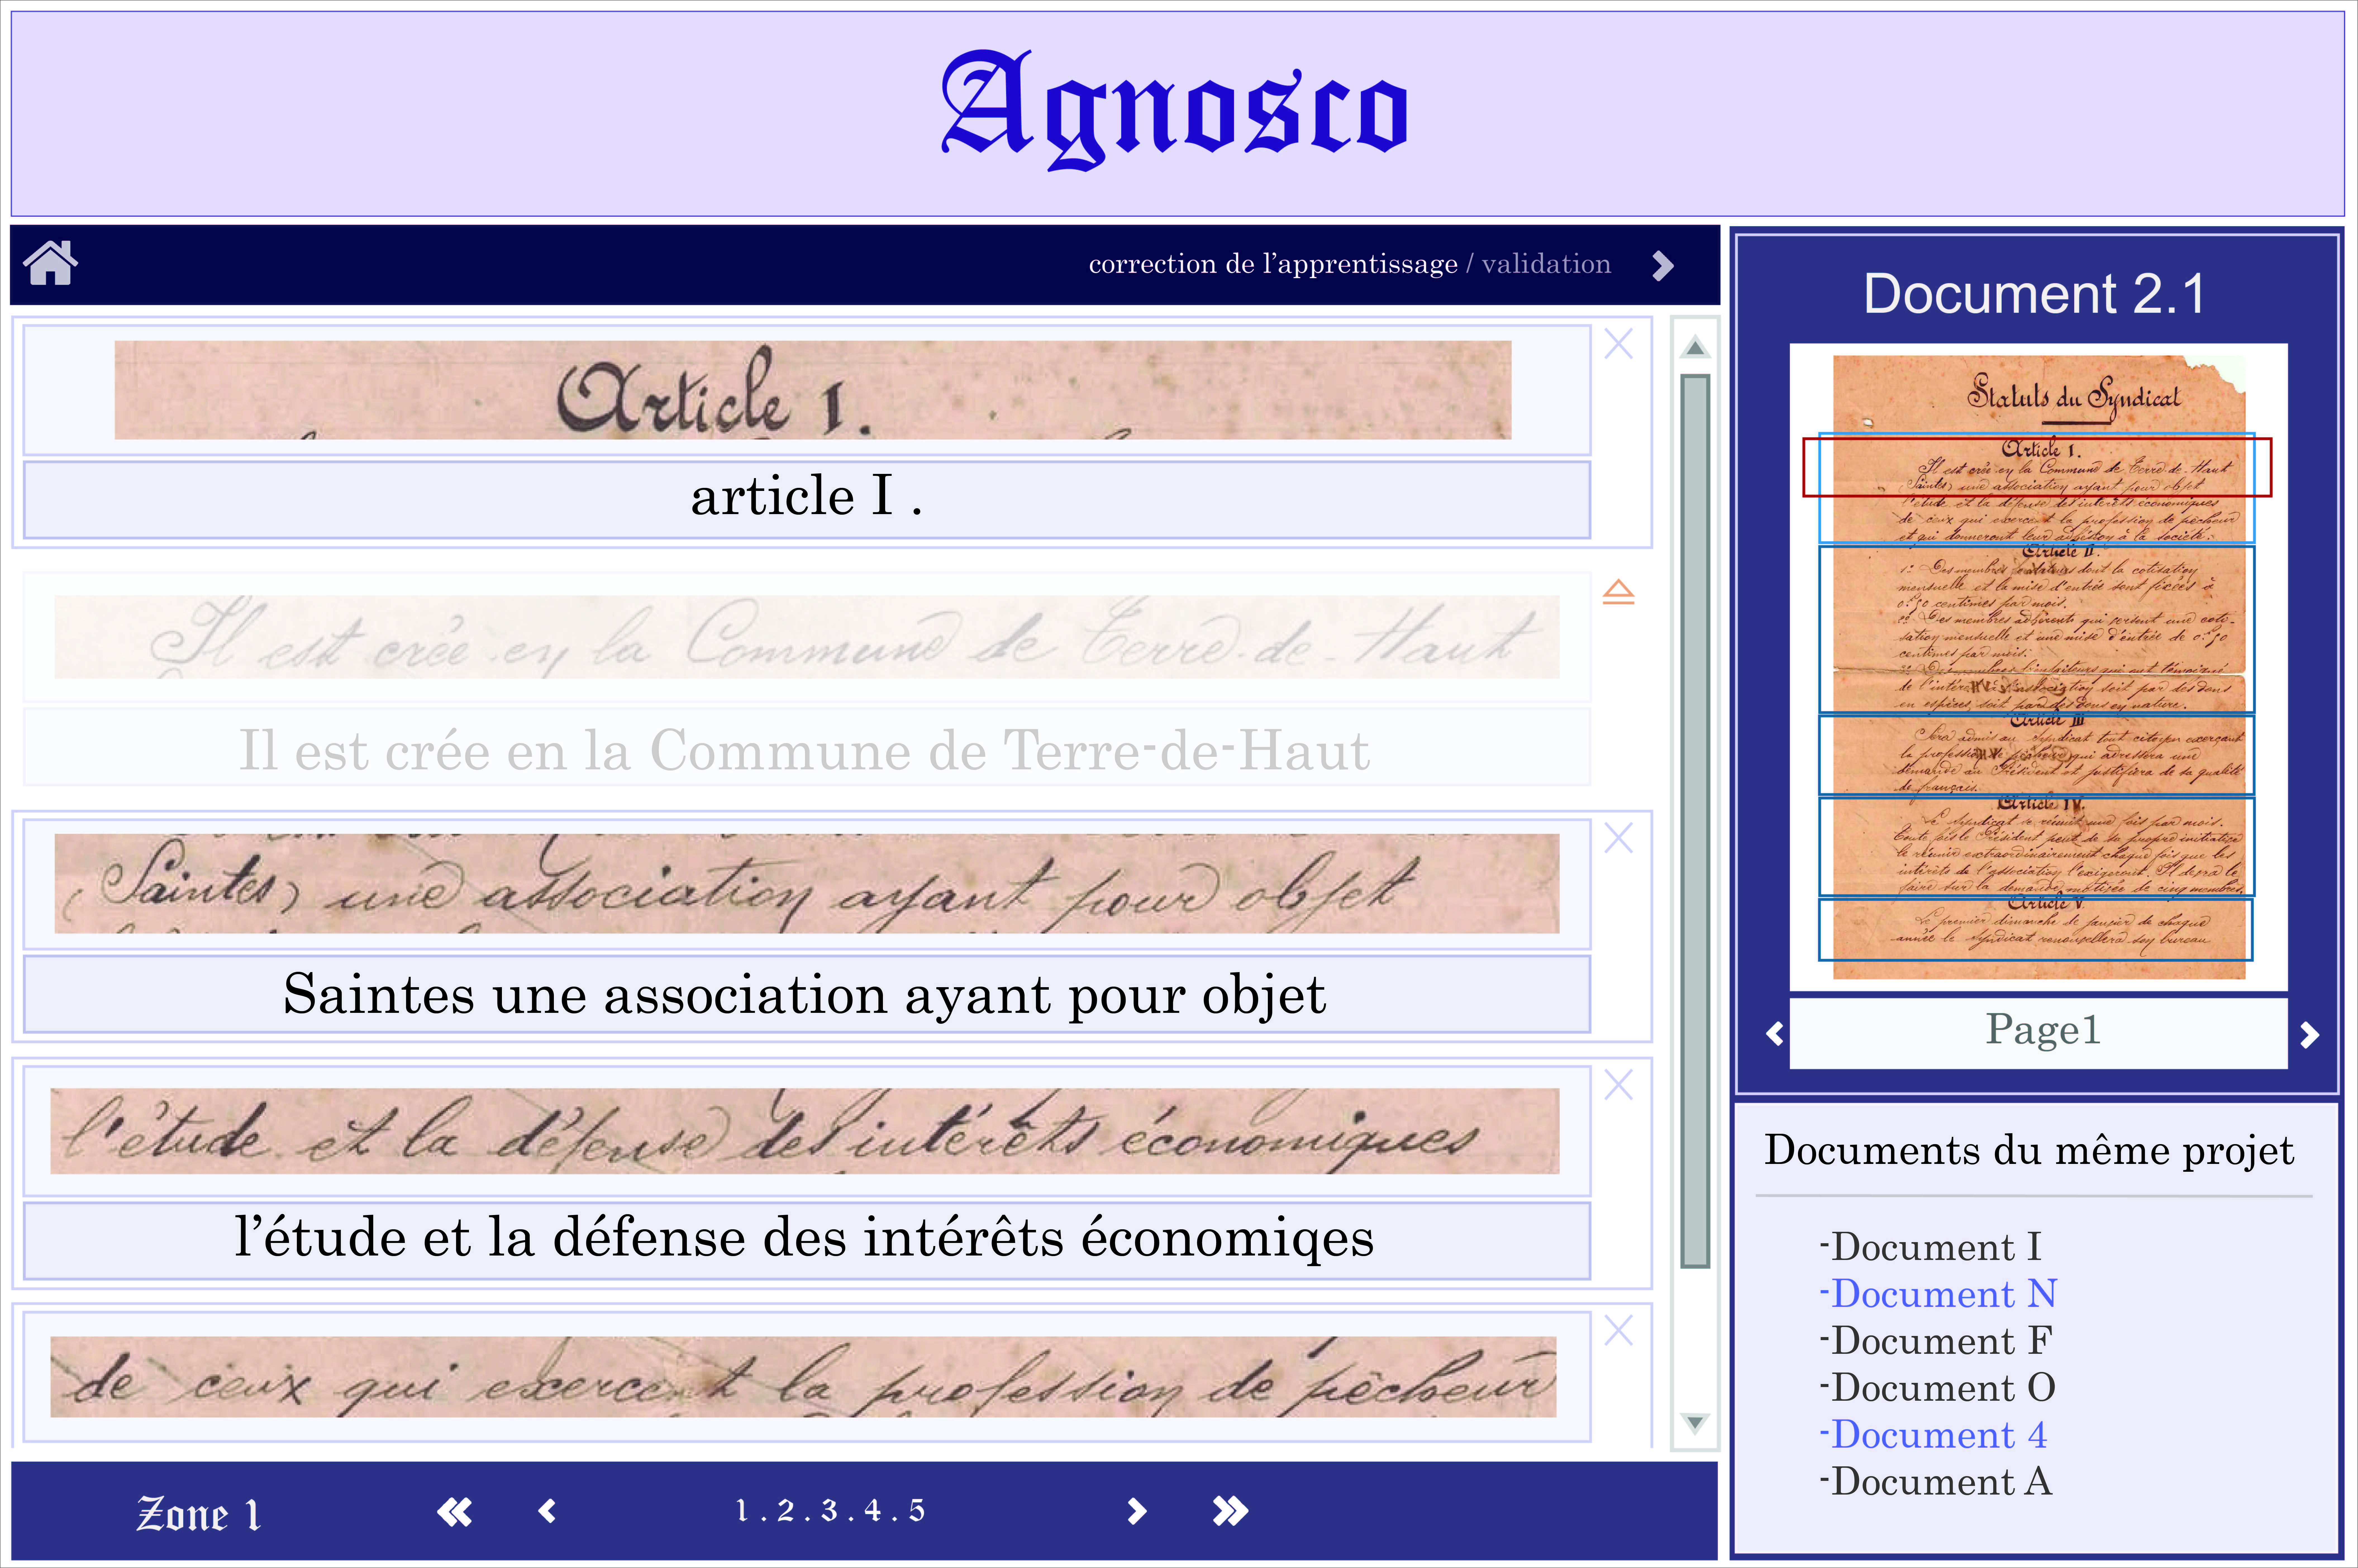
\includegraphics[scale=0.05]{ihm4.jpg}
\end{center}
\end{mdframed}

\subsection{Mode validation}

La page de validation est l’étape finale du travail d’annotation d’un
manuscrit. Cette page est accessible depuis le menu principal, une fois que
l’utilisateur a choisi son manuscrit, afin qu’il puisse valider directement les
transcriptions existantes (\textbf{PVAL\_1}). Elle est également accessible
depuis les pages d’édition manuelle des annotations et de correction des
transcriptions proposées par le reconnaisseur (\textbf{PVAL\_2}).

\paragraph{}
En partant du principe que c’est une validation finale et que les
transcriptions sont donc censées être majoritairement correctes, l’interface
propose une lecture rapide pour ajouter des corrections si besoin. Ainsi, un
simple appui sur Entrée valide les transcriptions zone par zone
(\textbf{PVAL\_3}). Si une transcription s’avère fausse, l’utilisateur doit
pouvoir la modifier en cliquant dessus et en effectuant ses modifications
manuellement (\textbf{PVAL\_4}).  L’utilisateur peut naviguer entre les 
différentes zones et les différentes pages grâce aux boutons prévus à cet effet.

\paragraph{}
L’interface indique si les transcriptions ont été fournies manuellement par un
humain ou si elles proviennent d’un reconnaisseur (\textbf{PVAL\_5}). Si elles
ont été renseignées par un humain, elles sont théoriquement justes et
l’utilisateur sait donc qu’il doit plutôt se focaliser sur la découpe des
imagettes, pour vérifier si la détection de lignes a bien été faite.

\paragraph{}
Dans le coin supérieur droit figure une fenêtre montrant la page entière
découpée en zones avec la zone courante dans une couleur différente
(\textbf{PVAL\_6}). Cela permet à l’utilisateur de connaître à tout moment sa
position dans le manuscrit. Enfin, un bouton permet de valider le travail pour
de bon et de fermer le document (\textbf{PVAL\_7}).

\newpage

\begin{mdframed}[frametitle={Figure 10 : Validation}, innerbottommargin=10]
\begin{center}
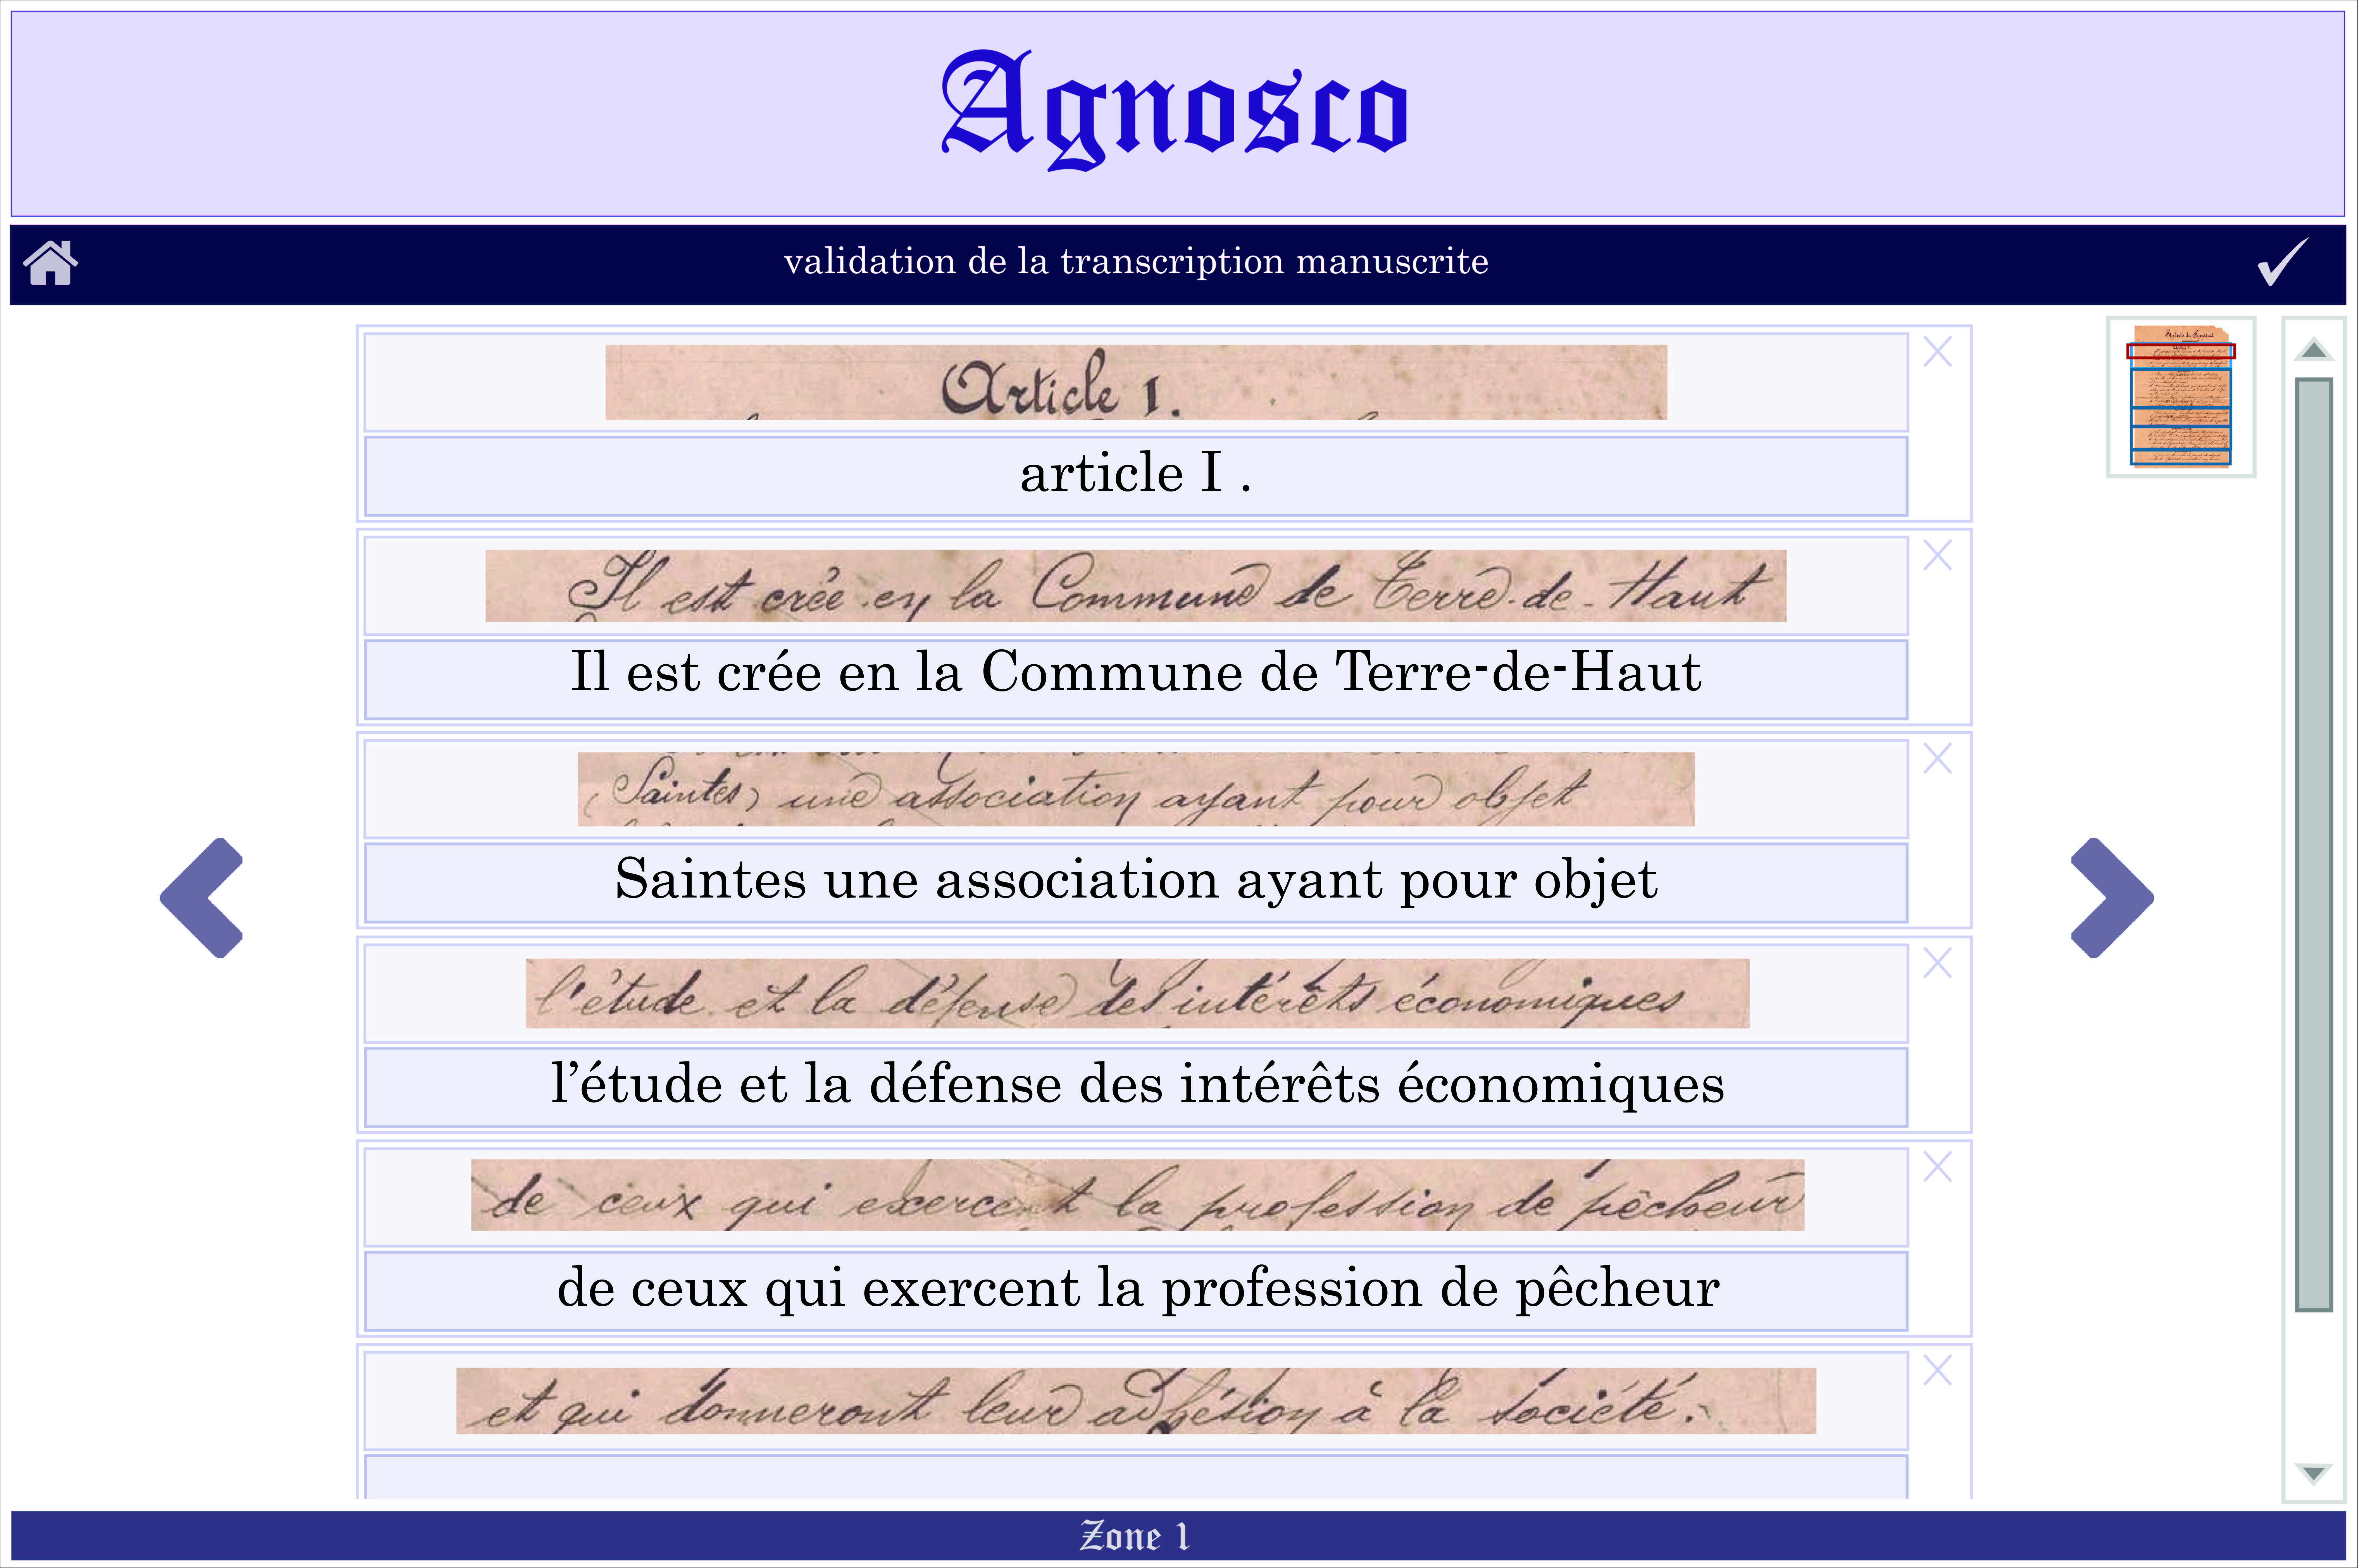
\includegraphics[scale=0.05]{ihm5.jpg}
\end{center}
\end{mdframed}

\subsection{Navigation dans l'application}

La navigation entre les pages de l’application se fait de manière la plus 
instinctive possible. Quand l’utilisateur ouvre l’application, il arrive 
sur la page d’accueil où il choisit son document, puis le mode de travail
 qu’il veut. La page correspondant au mode s’ouvre ensuite (édition manuelle 
des annotations, correction des propositions du reconnaisseur ou validation).
 L’utilisateur peut retourner au menu à tout moment à l’aide d’un bouton
 prévu à cet effet ou passer au mode de validation depuis les pages 
d’édition des annotations et de correction de la reconnaissance. De plus, 
la page d’édition des zones de découpe est accessible depuis la page 
d’annotation manuelle.

Lorsque l’utilisateur annote un document, il peut naviguer simplement 
dans ses différentes pages grâce à la barre de navigation située dans 
la zone à droite des imagettes où figure la page entière courante découpée.

Quand un document est en cours d’annotation, la navigation vers un autre 
document au sein du même projet se fait dans la zone “Documents du même 
projet”. L’utilisateur sélectionne le document qu’il veut ouvrir, 
choisit le mode de travail, puis le document s’ouvre.



